\section{Timeline}

The following section describes the project development, progress and decision as we did through the time the the project was developed. After series of informal talk the project officially started in December 2011 and was submitted in September 2012.

\subsection{Initial project meetings and early implementation decisions}

The regular project meeting where we discussed mostly the organizational aspects and the top-level design of the application started in December 2011. We easily agreed that we were aiming to create an application quite similar to the Google Documents. We have decided very early to use the multi tier architecture consisting of

\begin{itemize}
\item core translation memory,
\item userspace,
\item graphical user interface,
\end{itemize}

which became very soon separate Maven modules. Although we added further modules later, we consistently kept the initial project splitting into \emph{Core}, \emph{User Space} and \emph{GUI}. At the beginning we also assigned team members to the different part of project which remained surprisingly stable as well. 

Before receiving the data from OpenSubtitles.org we were thinking about the source of data to fill the translation memory for the first time. There were several options -- either using the subtitle part of the Czech-English parallel corpus CzEng developed at ÚFAL, using sentences from a general purpose parallel corpus or getting the data from a subtitle server.

From the very beginning we intended base the project on Java. Mainly because there exist quite a lot of web technologies based on Java and everybody of us were at least a little bit familiar with it. We also decided to combine the code in Java and Scala programming languages and Apache Maven as a build manager.

Much complicated was to agree on the technology of the client. There were many different opinions from writing the client in {\it PHP} with {\it Nette Framework} which some of us know, using the {\it JSP} to have all the code consistently in Java or even quite extreme idea to make the whole application as {\it Java Applet} (it was because of the intention to integrate the video player in the application). Finally we decided to use {\it Google Web Toolkit} which nobody of us had had any prior knowledge before, but it promised making the communication between server and client very easy.

After overcoming the problems connected with learning a new technology we became quite satisfied with the decisions because the usage of Google Web Toolkit and other modules, as well as the possibility to combine all parts of the project with Apache Maven were helpful despite making the project run in Maven was very painful for us and we spent unnecessarily a lot of time by solving this issues.
	
The decision to use both Java and Scala appeared to be a bring quite a lot of complications. On the one hand, Scala allowed to write concise and efficient code, on the other hand most project members were not able to learn Scala sufficiently and hence used only Java. Although the interoperability between Scala and Java works well in most cases because both are based on the JVM, some problems remain. One of the problems of interoperability was, for example, that the implementation of the data type \emph{List} that was created in Scala was not compatible with Google Web Toolkit, which expected a standard Java \emph{List} implementation.

\subsection{Early development process}

Luckily for us we received very soon a database from the {\it opensubtitles.org} containing all the Czech and English subtitle file that were at the server at that time. Soon after that we started an alignment algorithm to retrieve the parallel data from the subtitle files (the process is described in section~\ref{sec:aligning_subtitles}) and enable us to start experiments that helped us to decide which database system could be used.

Choosing appropriate database system was also intensively discussed issue. The database underlying the Translation Memory plays a crucial role for the whole system performance. Also using built-in features could save us a lot of additional work.  We evaluated different DBMS and decided to use Postgres (see section~\ref{sec:dbms} for details).

Originally, all the algorithms precessing the data we retrieved were implemented in Perl the and the code importing the data were in the \emph{Core} module implemented in Scala. Later, to be the code more consistent, we decided to move the data preparation and data import to a separate \emph{dataimport} module and re-implement the Perl scripts in Scala.

\begin{figure}[h]
\begin{center}
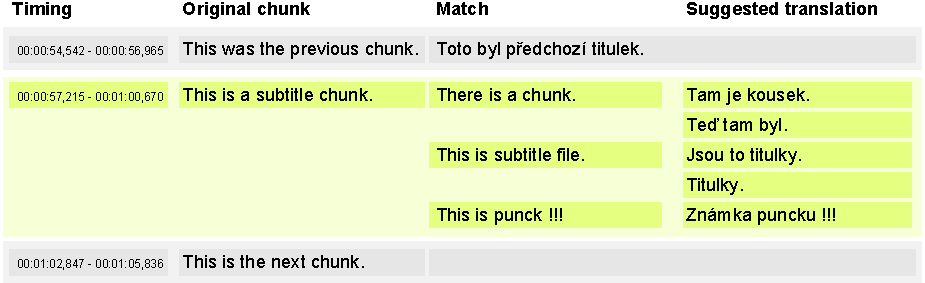
\includegraphics{./figures/original_strucutre.pdf}
\end{center}

\caption{Scheme of the originally intended structure of work with the translation memory. It reflects the original User Space structure and also schematically the original client design.}

\end{figure}

\subsection{Agreement on shared classes}

After having implemented basics of everything ... Crucial moment 

\begin{itemize}
	\item We agreed on the shared classes that all parts of the project should use. For best compatibility between  \emph{Core}, \emph{Userspace} and the GWT-based \emph{GUI}, we decided to write all shared classes in Java.
\end{itemize}


\noindent\textbf{Discussion of the decision}

\begin{itemize}
	\item It showed to be an important decision to agree on the shared classes early in the project since it made the cooperation between the modules easier and less verbose.
\end{itemize}


\subsection{Core design decisions}



\subsection{User Space design decisions}



\subsection{GUI design decisions}

\section{Evaluating the Development Process}

One of the crucial decision for the project was the choice of technologies. Most of the technologies we used -- Maven, Scala, Hibernate, GWT -- were new to all of us and we also had not much experience with the other. Combining these technologies together was quite painful and would probably even for an experienced Java developer. Generally, we can say that the fact that we were not too much familiar with the technologies, we spent most of the time solving technical issues. There is quite a lot of research challenges, mostly in the fuzzy matching part, which had to remain untouched due to that.

On the other hand the choice of technologies appeared to be lucky that it probably saved a lot of work for us by the possibility to share implementation of class. Using the Scala language for the core also made the parallelization much easier.

Despite we spent quite a lot of time by the discussions how the structure of the project we didn't avoid a radical change of the design of the application 4 months after the project started. Nearly the whole User Space code had to be dropped and it was also necessary to totally remake the client components existing so far.





